\documentclass{sig-alternate}

\usepackage{graphicx}
\usepackage{listings}

% For appendix:
\usepackage{pdfpages}
\usepackage{fancyhdr}

\usepackage{url}
\usepackage{hyperref}
\hypersetup{breaklinks}

\begin{document}
\title{Gear Smarts - A Machine Learning Approach to Outdoor Activity Outfit Selection}
\author{Ross Nordstrom\\
        University of Colorado - Colorado Springs\\
        1420 Austin Bluffs Pkwy,\\
        Colorado Springs, CO 80918\\
        \texttt{rnordstr@uccs.edu}
        \texttt{nordstrom.ross@gmail.com}
       }
\date{March 30, 2015}

\maketitle

\begin{abstract}
This paper explores the use of machine learning classification, along with an API-consuming infrastructure, to
produce clothing suggestions for outdoor activities based on an activity and the weather. The focus will be an
application for suggesting which layers to wear before going out to ski or snow board.
\end{abstract}

% See http://cran.r-project.org/web/classifications/ACM.html
% This might need to be changed if I narrow in or switch specific ML methodology
\category{I.2.6}{Computing Methodologies}{Artifical Intelligence - Learning}

\terms{Machine Learning}
\keywords{Machine Learning, Artificial Intelligence, Knowledge Database}

\section{Motivation}
\label{section:motivation}
This proposal seeks to implement a tool or application to assist in the selection of what to wear based on
historical data, an activity, and a locale (or weather). The purpose of this project is to use a real-world
problem to drive the use of machine learning in an integrated system. Originally, the project idea came from trying
to decide which layers to wear by recalling what was used before in similar weather conditions. This is a
useful and intersting application of machine learning because it has real-world value and is extensible to a variety
of areas, including a variety of sports or activites, or what to pack for a vacation.

\subsection{Value}
Many outdoor activities, such as skiing, require planning ahead for the entire day. An especially important
decision is what to wear, or more specifically what layers to wear (e.g. a base layer, a fleece jacket, and a shell).
This decision is strongly dependent on several variables, including the temperature throughout the day, the weather
quality (sunny, cloudy, snowing), and even which specific activity will be done (such as mogul runs or groomers).
Additionally, a person's ``mental repository'' indexing what they've worn in the past for similar weather conditions
may be sparse due to infrequently taking part in the activity, or conducting the activity in a new environment (e.g.
after moving).

If there were a tool to help apply a person's own history as well as that of similar users to a given day's weather
forecast, the decision could become easy.

\subsection{Extensibility}
This use of machine learning is applicable to anyone venturing into variable climates and/or activities.
By quickly and simply categorizing
users and their current locality, we could develop an ever-growing database of (1) items to wear and their properties,
(2) user types (i.e. cold/heat tolerance), and (3) characteristics of various weather types (think windchill).

\subsection{Market}
In general, there has been an explosion in the popularity of apps and products surrounding sports and outdoor activities.
Of note is the EpicMix application and infrastructure \cite{EpicMix:Site}, which helps hundreds of thousands of skiers and snow
boarders \cite{EpicMix:PlayStore} gain insight into how much they are skiing by tracking and gamifying the lifts they ride up.
Other industries, especially running and hiking, have experienced a large growth in the use of technology to augment and
track user experience. With users becoming more accustomed to the use of technology to augment their participation in outdoor
activities, there has never been a better time for a tool targeted at helping people decide how to gear up for the day.

\section{Related Work}
\label{section:relatedwork}
While there have been a number of works in automating outfit selection, they are all geared towards
fashion selection either for aesthetics or occasions (e.g. wedding, funeral, interview, or church).
There does not seem to be any existing work in the climate-outfitting field, let alone with an
activity focus.

In general, related works fall into three categories: fashionable outfit selection, category-based
outfit selection, and general temperature/climate automation. Here several related works are briefly introduced:

\subsection{Fashionable Outfit Selection}
\cite{Dressup} uses a wardrobe of known clothes to suggest outfits based on the user's appearance.
Of note is that outfits are suggested based on a dress code constraint, which is a similar task to
the challenge of outfit selection.

Yu et al. \cite{SmartCloset} works on outfit selection and sharing, focused on comparing and lending wardrobe
to others. There may be some similarities between this and the idea of comparing user outfit preferences
for Gear Smarts.

Rode et al. \cite{MagicCloset} used Amazon's Mechanical Turk to fill a database of available-to-purchase outfits.
Using this dataset, they constructed an occasion-oriented outfit suggestion tool similar to \cite{Dressup}.

Liu et al. \cite{ThermalComfort} discusses a new approach to thermal control of homes. This could relate well to
adapting Gear Smarts to sub-activities with different thermal properties (e.g. mogul vs groomer skiing).

\subsection{Machine Learning Technique Selection}
There are numerous papers discussing and comparing the various options for machine learning techniques.
Some relevant papers to the decision of which technique to use for Gear Smarts include \cite{ML:MapReduceClusters},
Clear et al. \cite{ML:ManufacturingSystems}, \cite{ML:IPTraffic}, and \cite{ML:GeoMapping}.

\section{Design}
\label{section:design}
To develop a climate and activity based outfit suggestion tool, the problem has been broken into parts.
At its core is a machine learning algorithm along with a datastore for the training data. Wrapping that is
a query system and eventually a mobile app for training the system. Additionally, an outfit modeller and persistence
engine will be implemented based on experience from evaluating the system by hand.
In this section, the envisioned parts of the system are presented. Note, this is the vision for the system as a whole and
not all components have been implemented for this report.

\subsection{Learning Core}
Support Vector Machines (SVMs) \cite{SVM} were chosen as the machine learning method for implementing an outfit predictor.
Justification for this choice is provided in Section \ref{section:mlsvm}. The learning core was implemented as a Node.js RESTful API to make it easy for a
Mobile App or Web UI to consume on behalf of users of GearSmarts. It has the additional benefit of being very easy to
script against, something that made evaluation of the tool much more approachable.
The API is described below in Section \ref{section:mlapi}.

\subsubsection{Justification for SVM}
\label{section:mlsvm}
Support Vector Machines were chosen over alternative machine learning methods for three main reasons.

Firstly, SVMs are built for classification problems and can be configured in a number of ways (such as linear vs.
nonlinear classifying) to make it applicable to a wider variety of problems than other methods might allow. This is
ideal for GearSmarts since we are exploring the problem space as much as solving it. The flexibility of SVMs will
help us react to changing or perhaps surprising discoveries.

The second reason for using SVMs is there is already an easy-to-use Node.js implementation library, \texttt{node-svm}
\cite{Github:nodesvm}. Since the details of implementing SVM are abstracted away, all we need concern ourselves with in
the GearSmarts API is normalizing and namespacing the datasets provided by consumers. Even better, \texttt{node-svm}
simply uses LIBSVM \cite{lib:libsvm}, which has been ported to or exposed in most major languages. The
widespread availability of this library means GearSmarts could be easily ported as-is to any of those languages.

Thirdly, the author already had experience with popular machine learning methods like Aritificial Neural Networks, and
Decision Trees. Support vector machines offer an opportunity to learn a new method and compare it to experiences with
other methods.

\subsubsection{Collecting Data}
In lieu of having a UI for users to train the system, a Google Form questionairre (included in Appendix
\ref{appendix:comfort_form}) was created for
friends and family to contribute datapoints. The response dataset includes about 50 datapoints (Appendix \ref{appendix:comfort_responses}).

Since the responses were provided in a clear-text and ``human'' format, they were reformatted by hand into a CSV format
starting with a class (``good'', ``cold'', ``hott'') and a locale descriptor, followed by activity, demographic, and
outfit features. To overcome the limited dataset size, the polled responses were duplicated and altered to produce ``obvious''
comfort classifications. For example if a person is hot in an outfit, adding more layers to it will still be hott.
Likewise, a ``common sense'' approach was used to fill in the opposite comfort class. For example, it's safe to say anybody
would be hot in three coats on a 70-degree day, and that anybody would be cold in a T-shirt on a 5-degree day.
More details on the data normalization process are discussed in Section \ref{subsection:preprocessing}

Regardless of the data collected for the outfit-specific problem, GearSmarts capabilities can be estimated by evaluating
it with published classification datasets, discussed in Section \ref{subsection:publicdatasets}. By assuring that the API
is capable of learning once the trained dataset is large enough, the target of outfit comfort classification
can be mastered more gradually over time with use of the system.

\subsubsection{Machine Learning RESTful API}
\label{section:mlapi}
In order to make GearSmarts as extensible and usable as possible, the machine learning core was implemented in Node.js
as a RESTful server, exposing two key routes describe below.

\begin{description}
    \item{\texttt{/v1/machinelearning/:namespace/train/:classification}} - Train the classifier on a single feature vector
    \item{\texttt{/v1/machinelearning/:namespace/classify}} - Classify a single feature vector
\end{description}

Both routes take a \texttt{:namespace} argument, which is simply an extensibility mechanism allowing consumers to train
many distinct datasets. For example, consumers training the \texttt{candy} namespace would not affect consumers training
the \texttt{fruits} namespace.

Additionally, each route expects a \texttt{POST} body or \texttt{GET} query containing an array of features to
train or classify under the \texttt{features} property. Interaction with a GearSmarts server is as simple as
making an HTTP call. An example of a training call is shown presently:

\begin{lstlisting}
http://localhost:8080/v1/ml/outfits/train/good
?features="['ski','groomers','meantempi=40',
'snow_pants','base_top','base_bottom','shell']"
\end{lstlisting}



In order to normalize the dataset, the server puts features into a dictionary of known features and uses their index
in the list for the SVM. The same combination of dictionary and indexing is used for the classifications too. This approach
was taken because the SVM library requires integer inputs. Examples of the dictionaries are shown in table
\ref{table:dictionary} and table \ref{table:datarow}. As an additional note,
trained data rows are stored in the API to more easily reason over the produced SVM. This storage currently lives in
memory only, but would eventually be moved to a database of some sort for persistence in a productized GearSmarts.
This data store would also make it easy to query and search outfits in use towards the marketing goals mentioned in
Section \ref{section:market}.

\begin{table}
    \begin{tabular}{lll}
        \hline
        \multicolumn{3}{c}{Classifications} \\
        \hline
        0 & 1 & 2 \\
        hott & good & cold \\
        \hline
        \hline
    \end{tabular}
    \begin{tabular}{lll}
        \multicolumn{3}{c}{Features} \\
        \hline
        0 & 1 & 2 \\
        meantempi=35 & snowpants & ... \\
        \hline
    \end{tabular}
    \caption{The SVM prefers integer classifications and features, so GearSmarts stores an Array of known classes and features,
    and uses their indexes in the SVM}
    \label{table:dictionary}
\end{table}

\begin{table}
    \begin{tabular}{llllr}
        \hline
        \multicolumn{5}{c}{Trained Data} \\
        \multicolumn{4}{c}{Features} & Class \\
        \hline
        ski     & downCoat  & helmet      & temp=25  & 0 \\
        iceFish & downParka  & woolHat      & temp=20  & 2 \\
        hike    & tshirt & temp=70  & & 1 \\
        \hline
    \end{tabular}
    \caption{The dataset is stored as a table with an Array of feature names and Array of Arrays of feature values. Note that rows
    do not need to have consistent feature vector sizes.}
    \label{table:datarow}
\end{table}

Along with the main classifier routes, GearSmarts also supports the querying of weather data using Wunderground \cite{wunderground}.
The route is accessed with a simple HTTP GET including a location and date, shown below. To reduce usage of Wunderground's limited
free tier API, all queries are cached on the filesystem. This has the additional benefit of making the usage of the weather info
easy to use in evaluation scripts.

\begin{description}
    \item{\texttt{/v1/weather?date=12/31/2014\&region=CO\&city=Colorado Springs}} - Get weather for a given date and place
\end{description}

\subsection{Problem Modeling}
Before using a machine learning system, the problem needed to be modeled properly. It can be broken down into three
fundamental parts, described below.

\begin{description}
  \item{Outfit:} Outfits can either be modeled individually or as a summation of individual articles (potentially introducing
  a knapsack problem\footnote{The knapsack problem seeks to optimize a value by searching combinations of a set. In GearSmarts,
  we might represent an outfit with a KPI that should closely match a KPI produced by a function of the weather. Meanwhile, each
  article of clothing in a wardrobe could have a KPI suggesting how warm it is. To properly match the knapsack problem, we might
  introduce a mobility metric for each article.}).
  Additionally, they can be represented categorically (e.g. vest or full-zip and
  fleece, down, and cotton) or by derived characteristics (e.g. thermal retention, mobility, wind-resistance).
  \item{Weather:} Weather should likely be characterized in terms of temperature, humidity, wind, atmospheric pressure,
  cloud cover, and precipitation.
  \item{Comfort:} Intuitively, there are three basic comfort levels relevant to GearSmarts: too cold, comfortable, and too hot.
\end{description}

Although a KPI\footnote{Key Performance Indicator (KPI) is a numerical representation of a problem space. These are often used to represent
complex problems in a single number for trending, tracking, or analyzing.} could be used to make the system more extensible, GearSmarts models the problem as a set of
articles of clothing, along with a true/false value for each. The UI will submit a list of articles the user wore (or
plans to wear) to the API, which maintains a dictionary (described above \ref{table:dictionary}) of known articles. The
API then normalizes the provided articles against the dictionary, producing a key/value object where the values are
simply \texttt{true} or \texttt{false} denoting if each is present.

Weather data is queried through the GearSmarts API as a key/value object of important
weather attributes in exchange for the consumer-provided location and date. The resulting key/value object should be
normalized by the consumer before being merged with outfit features to construct a feature vector. More details about
the normalization process used for this report are discussed in Section \ref{section:evaluation}. As is typical in
machine learning, the technique used to normalize the features has an enormous impact on the effectiveness of the
classifier.

The comfort level would be selected from a static list of options (``hot,'' ``cold,'' and ``good'') by the user when
training the system. When the UI tries to make an outfit suggestion, it would search the available set of articles of
clothing (a ``wardrobe'') combined with the known weather features, querying the machine learning \texttt{/classify}
route to find a subset of the wardrobe with a ``good'' classification.

\section{Objectives and Timeline}
\label{section:objectives}
This project intends to apply machine learning to a real-world use case to improve understanding of
how to apply the theory. Interestingly, Gear Smarts, as so far proposed, will feature several other engineering
problems in addition to implementing a machine learning technique. Deadlines, achieved and pending, are described in a
table to help pace the project during the semester \ref{table:objectives}.

\begin{table}
    \begin{tabular}{llc}
        \hline
        \textbf{Task} & \textbf{Risks} & \textbf{Deadline} \\ [0.5ex]
        \hline\hline
        Determine ML technique & - & - \\
        \hline
        Implement ML technique & - & - \\
        \hline
        Define outfit modeling & - & - \\
        \hline
        Midterm & - & - \\
        \hline
        Weather API & See \cite{API:OpenWeatherMap} & [Slipped] APR-06 \\
        \hline
        UI App/Site & Minimal & APR-13 \\
        \hline
        Evaluation of work & Minimal & APR-27 \\
        \hline
        Final & - & MAY-06 \\
        \hline
    \end{tabular}
    \caption{Deadlines throughout the semester to ensure the success of the project. ``-'' denotes completed tasks.
    All dates are for the year 2015.}
    \label{table:objectives}
\end{table}

% \section{Implementation}
\label{section:implementation}
[implementation here]

\subsection{Some subsection}
[subsection here]

% \section{Future Work}
\label{section:futurework}
As the vision of GearSmarts was described in Section \ref{section:design}, the main missing components are simply a UI
and searching for an optimal outfit out of a given wardrobe. Additionally there is room to improve the classifier and
understanding of the outfit comfort problem modeling.

\subsection{User Interface}
\label{section:ui}
While it was appropriate to simply use scripts for the initial evaluation and implementation of the GearSmarts API for
this report, eventual productization of the tool will require a UI with which users can easily use the API. The vision
for the UI is that it will store and model a user's wardrobe (their collection of known articles of clothing), against
which it can search combinations for the optimal outfit for a given activity in queried weather for the desired location
and date. Additionally, the UI should make it easy and enjoyable for users to log their outfits and comfort level in order
to train the system. The best approach is likely to gameify it somehow so that users are rewarded for recording more
data, thus better training GearSmarts more.

\subsection{Modeling and Configuration}
\label{section:modelingandconfig}
As this application of machine learning is exploratory, the approach taken for modeling the problem space, the
SVM configuration used, and the weather data selected in GearSmarts is expected to evolve as more data is collected and
a better understanding of the problem space is acquired. Additonal steps and layers may be beneficial to the system, such
as clustering users into groups of similar heat-tolerances. Then each of these clusters could be trained and classified in
their own namespace in GearSmarts, thus isolating the ``run-hot'' from the ``always-cold'' users.
% \section{Conclusion}
\label{section:conclusion}
The vision and design initially proposed for GearSmarts turned out to be achievable, but with some room for improvement
with more experience and data collection. Overall, the architecture of the system turned out to be extensible enough to
support a variety of independent evaluations, while being both performant and easy-to-use. While the project fell short
in some areas relative to the vision (specifically the lack of UI), it did not impact our ability to evaluate GearSmarts.

\bibliography{citations}{}
\bibliographystyle{acm}

\clearpage
\section{Appendix}
\label{appendix}

\subsection{Comfort Level Form and Responses}
\label{appendix:comfort}
Attached here is a Google Form which was shared with the author's friends and family to collect data about their
comfort levels during activites. Also attached is a spreadsheet of the responses collected from the questionairre.


\begin{figure}[ht!]
    \centering
    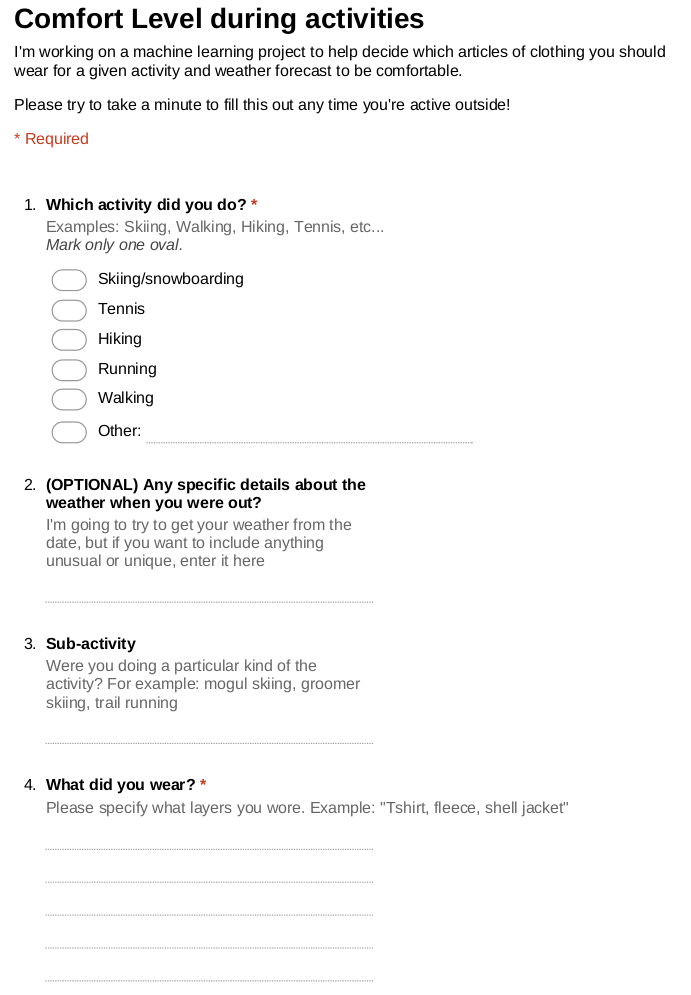
\includegraphics[width=90mm]{img/survey.png}
    \label{appendix:comfort_form}
\end{figure}

\label{appendix:comfort_responses}
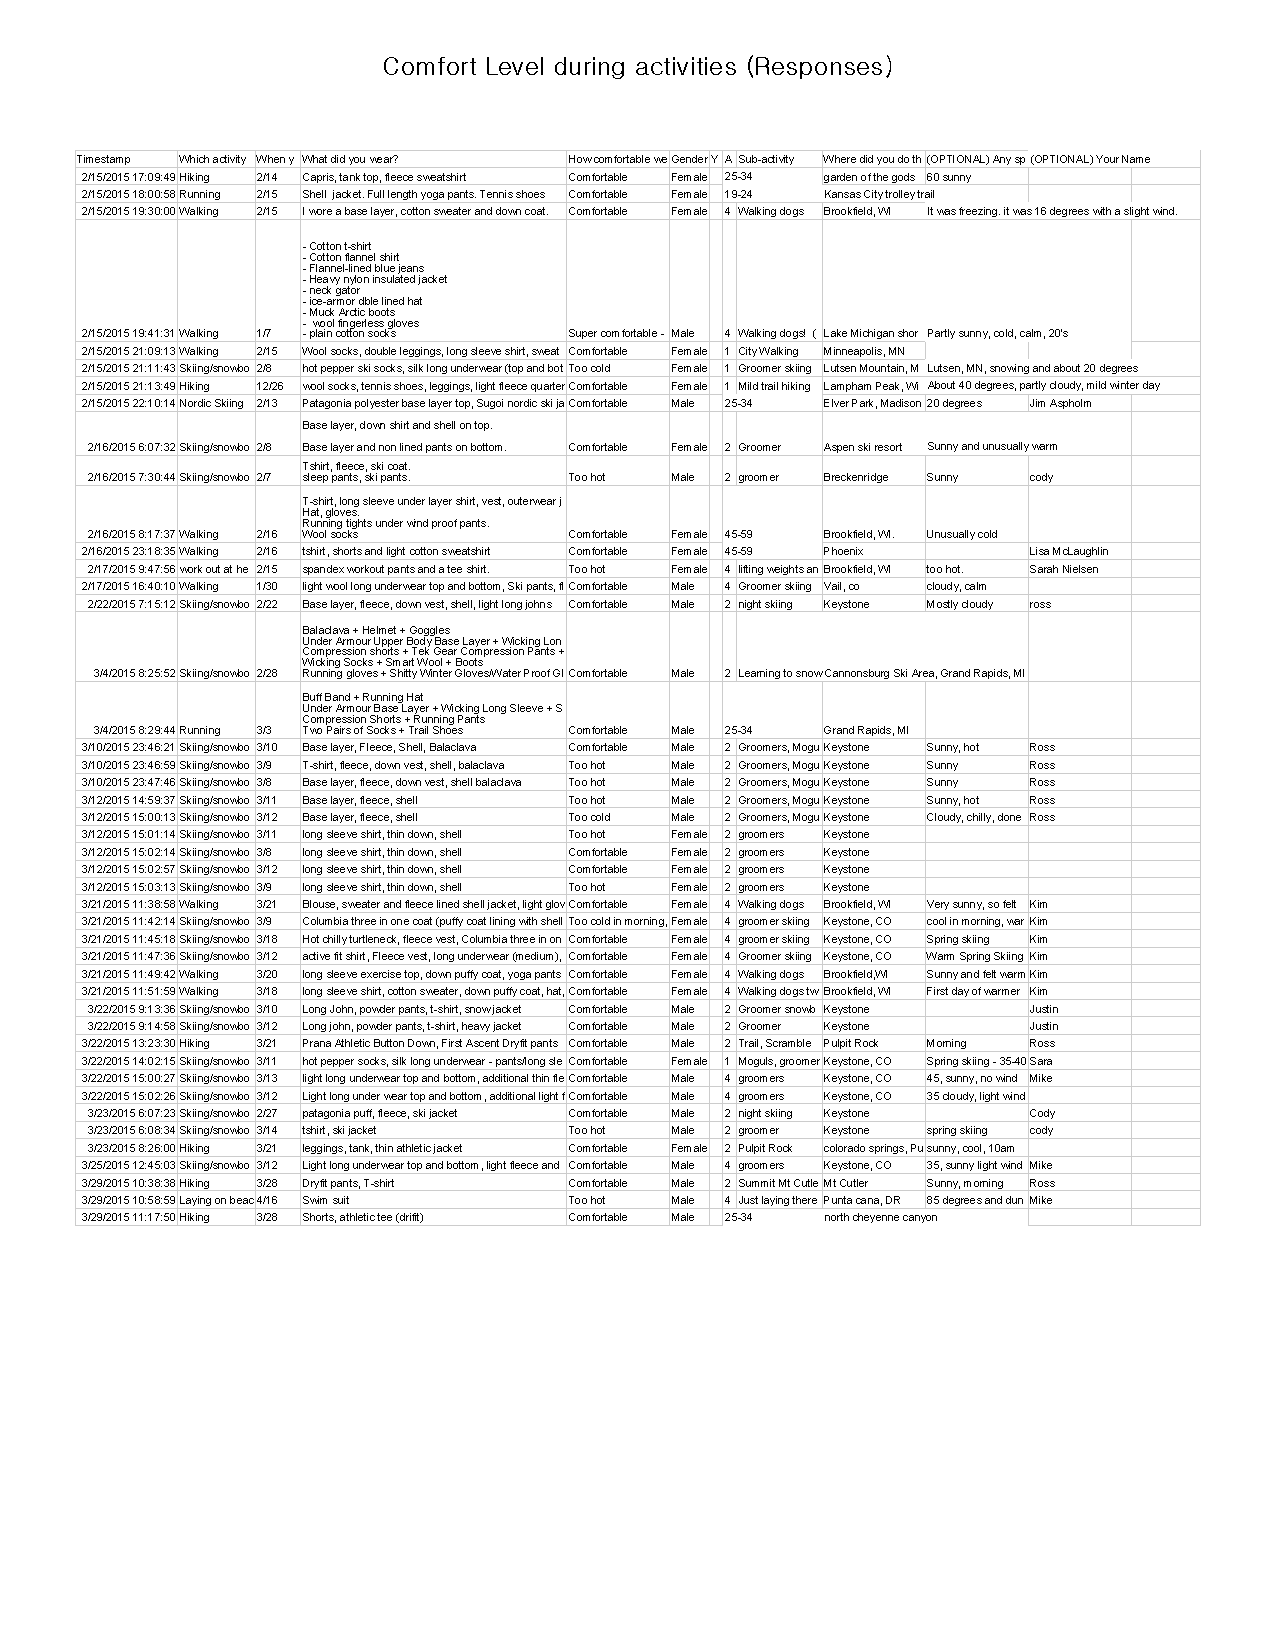
\includepdf[pages=1,
            pagecommand={\thispagestyle{fancy}},
            width=\textwidth,
            frame]{appendix/ComfortLevel_responses.pdf}



\end{document}
